\newcommand\thC{\(\theta^1\)\,Ori~C}
\defcitealias{Canto:1996}{CRW}
\newcommand\CRW{\citetalias{Canto:1996}}

\section{Hypersonic thin shell model}
\label{sec:crw-scenario}
This scenario can be described with the formalism of
\citet[][hereafter \CRW{}]{Canto:1996}, who proposes an algebraic
solution for the two winds interaction problem in the thin shell
approximation, in terms of a free parameter
$\beta\equiv\frac{\dot{M}_wv_w}{\dot{M}_{w1}v_{w1}}$, the winds
momentum ratio, which the quantities with subindex 1 corresponds to
the strongest wind, therefore $\beta<=1$. In this work the weakest wind is modeled as an anisotropic hemispherical radial wind
with the following density distribution:

\begin{align}
  n(\theta) = n_0\cos^k\theta
\end{align}  
The index $k$ gives the anisotropy degree. We are interested in winds where $k \geq 0$ for further applications. By the other side, we keep the strongest
wind as isotropic.

The shape of the resultant bow shock is given by:
%If we apply the \CRW{} formalism for a more generalized photoevaporated flow with density given by (\ref{eq:ngen}),
%we find that the solutions for equations (8) - (11) of \CRW{} are the following:

%If we apply the \CRW{} formalism for a generalized photoevaporated flow with density given by equation (\ref{eq:ngen}),
%the shell shape $R(\theta)$ may be calculated from equation (6) of CRW{}:
\begin{align}
  R = \frac{\dot{J}_w + \dot{J}_{w1}}{\left(\dot{\Pi}_{wr}+\dot{\Pi}_{wr1}\right)\cos\theta-\left(\dot{\Pi}_{wz1}+\dot{\Pi}_{wz1}\right)\sin\theta}
  \label{eq:Rmom}
\end{align}

Where:

\begin{align}
\dot{\Pi}_z &= \frac{v_w\dot{M}_w^0}{2(k+2)}\left(1-\cos^{k+2}\theta\right)  \label{eq:pir}\\
\dot{\Pi}_r &= \frac{1}{2}\dot{M}^0_w v_w I_k (\theta) \label{eq:piz}\\
I_k(\theta) & = \int^\theta_0 \cos^k \theta \sin^2\theta~d\theta \\
\dot{J}_w = 0 \label{eq:jdot} \\
\dot{M}_w &= \frac{\dot{M}_w^0}{2(k+1)}\left(1-\cos^{k+1}\theta\right) \label{eq:dotprop} \\
M^0_w &\equiv 4\pi v_w r^2_{IF} n_0 \bar{m}\\
\dot{\Pi}_{wz1} & = -\frac{\dot{M}^0_{w1}v_{w1}}{4}\sin^2\theta_1\\
\dot{\Pi}_{wr1} & = \frac{\dot{M}^0_{w1}v_{w1}}{4}\left(\theta_1-\sin\theta_1\cos\theta_1\right)\\
\dot{J}_{w1} & = \frac{\dot{M}^0_{w1}v_{w1}}{4}\left(\theta_1-\sin\theta_1\cos\theta_1\right)D \label{eq:jdot1}
\end{align}

Combining equations  (\ref{eq:pir}) to (\ref{eq:jdot1}) we can obtain numerically the bow shock shape $R(\theta)$ from equation (\ref{eq:Rmom}).
To find the projected shape in the plane of sky, we fit $R(\theta)$ into a quadric curve which has the same characteristic radii $(R_0,R_c,R_{90})$. 
%The most notable scenarios, since they have astrophysical relevance are the following:
%$k=1/2$ ak.a. the ``proplyd case'', following \citep{HA:1998}, and $k=0$, ak.a, the ``isotropic case'', following \CRW{}. The comparison between both solutions
%is shown in figure (\ref{fig:r-beta}), along with an extreme anisotropy case. 

\begin{figure}
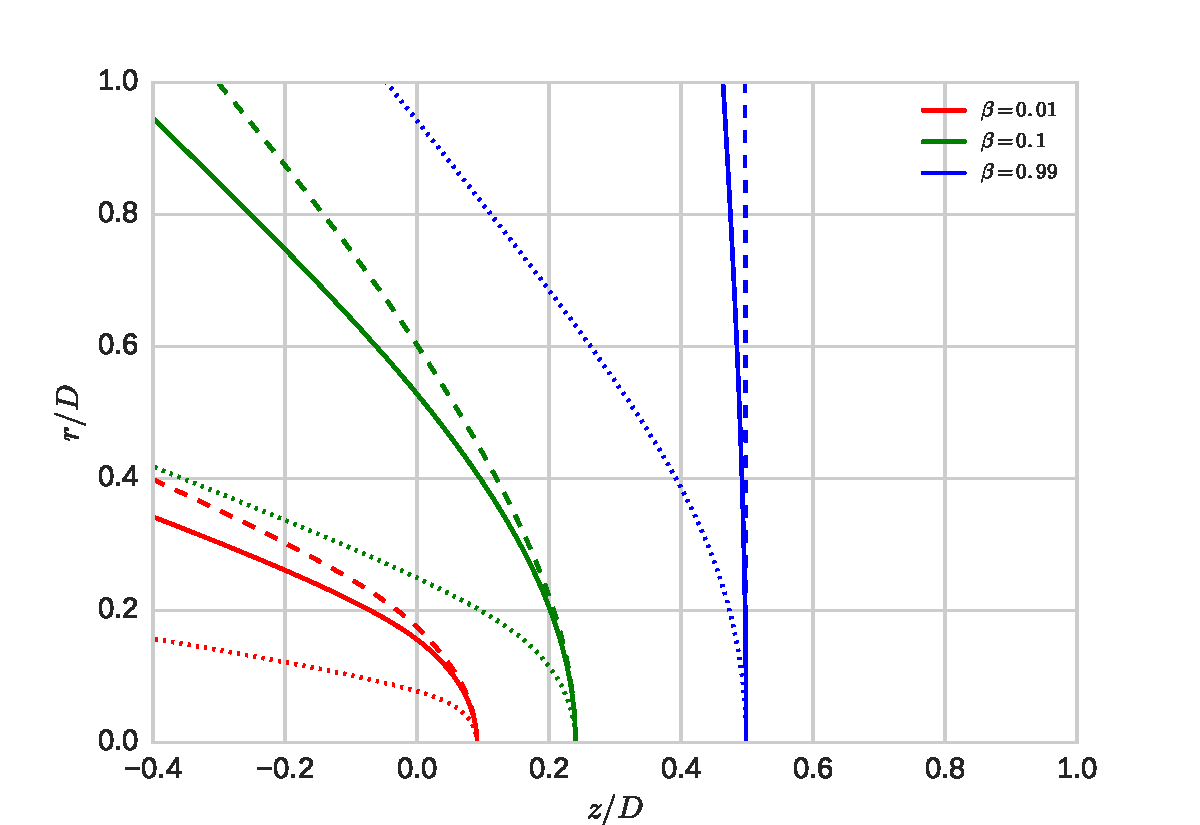
\includegraphics[width=\linewidth]{r-beta}
\caption{Bow shock shapes for interacting winds in the thin-shell
  approximation. Coordinates are normalized by $D$, the distance
  between the two wind sources.  The weaker source is at \((0.0, 0.0)\)
  and the stronger source is at \((1.0, 0.0)\).  Results are shown for
  different values of the wind momentum ratio, \(\beta\), and for the
  case where the weaker wind is isotropic (dashed lines) or an
  anisotropic photoevaporation flow. The solid lines shows a wind with a
  moderate degree of anisotropy $(k=0.5)$, which is expected for the proplyds.
  And the dooted lines show a wind with extreme anisotropy degree $(k=8)$.}
\label{fig:r-beta}
\end{figure}


\subsection{Characteristic Radii}
$R_0$ is obtained directly from equation (27) of \CRW{} as the distance from the inner source where the RAM pressure of the interacting winds is in equilibrium.
%Here goes a little introduction
For the rest of the radii we need a relation between $\theta$ and $\theta_1$ as follows:


\begin{align}
\theta_1\cot\theta_1 -1 = 2\beta I_k(\theta) \cot\theta - \frac{2\beta}{k+2}\left(1-\cos^{k+2}\theta\right)
\label{eq:th1th}
\end{align}

Equation (\ref{eq:th1th}) is reduced to equation (24) of \CRW{} when $k=0$.
We can obtain $R_{90}$ by the following process:
Evaluating equations  (\ref{eq:th1th}) and (23) from \CRW{} at $\theta=\frac{\pi}{2}$ we obtain the following:

\begin{align}
R_{90} = D\tan\theta_{1,90} \\
\theta_{1,90}\cot\theta_{1,90} = 1-\frac{2\beta}{k+2} \label{eq:th190}
\end{align}
Where $\theta_{1,90}\equiv \theta_1(\frac{\pi}{2})$. Combining both equations and  introducing the parameter 
$\xi\equiv \frac{2}{k+2}$ we have:

\begin{align}
R_{90} &= D\frac{\theta_{1,90}}{1-\xi\beta} 
\end{align}


Solving for $\theta_{1,90}$ from equation (\ref{eq:th190}), using a small angle  approximation, we find that:

\begin{align}
\theta_{1,90} &\simeq \left(\frac{3\xi\beta}{1+\frac{1}{5}\xi\beta}\right)^{1/2} \\
\label{eq:th190sol}
\end{align}

With this, we have a solution for $B \equiv \frac{R_{90}}{R_0}$:

\begin{align}
B = \frac{\sqrt(3\xi)\left(1+\beta^{1/2}\right)}{(1-\xi\beta)\left(1+\frac{1}{5}\xi\beta\right)^{1/2}}
\label{eq:B}
\end{align}

Now, to obtaining $R_c$ we expand  (\ref{eq:th1th}) until order 4th order for small $\theta$ values to find that for such values

\begin{align}
\theta_1^2 &\simeq \beta\theta^2\left[1+ 2C_{k\beta}\theta^2\right] \\
\mathrm{where:~} & C_{k\beta} \equiv \frac{1}{30}\left(1-\beta-\frac{9}{4}k\right)
\end{align}
Expanding equation (23) from \citep{Canto:1996} and substituting $\theta_1$ we found that:

\begin{align}
R &\simeq R_0 \left(1+\gamma\theta^2\right)
\label{eq:R_approx} \\
\mathrm{where:~} & \gamma = \frac{C_{k\beta}}{1+\beta^{1/2}}+\frac{1}{6}(1-2\beta^{1/2})
\end{align}

Which lead us to derive the radius of curvature at the symmetry axis:

\begin{equation}
R_c = R_0\left(1-2\gamma\right)^{-1}
\label{eq:Rcurv}
\end{equation}

finally, using equations (\ref{eq:Rcurv}) and (\ref{eq:B}) we can estimate the parameter of conic curves $\theta_c$ as a function of $(\beta,\xi)$ using equation (\ref{eq:thc-conic})

\begin{align}
\tan^2\theta_c &= \left| \frac{3\xi\left(1+\beta^{1/2}\right)^2}{\left(1-\xi\beta\right)^2\left(1+\frac{1}{5}\xi\beta\right)}-\frac{2}{\left(1-2\gamma\right)}\right| 
\label{eq:thc-CRW}
\end{align}

\begin{figure}
\begin{tabular}{c}
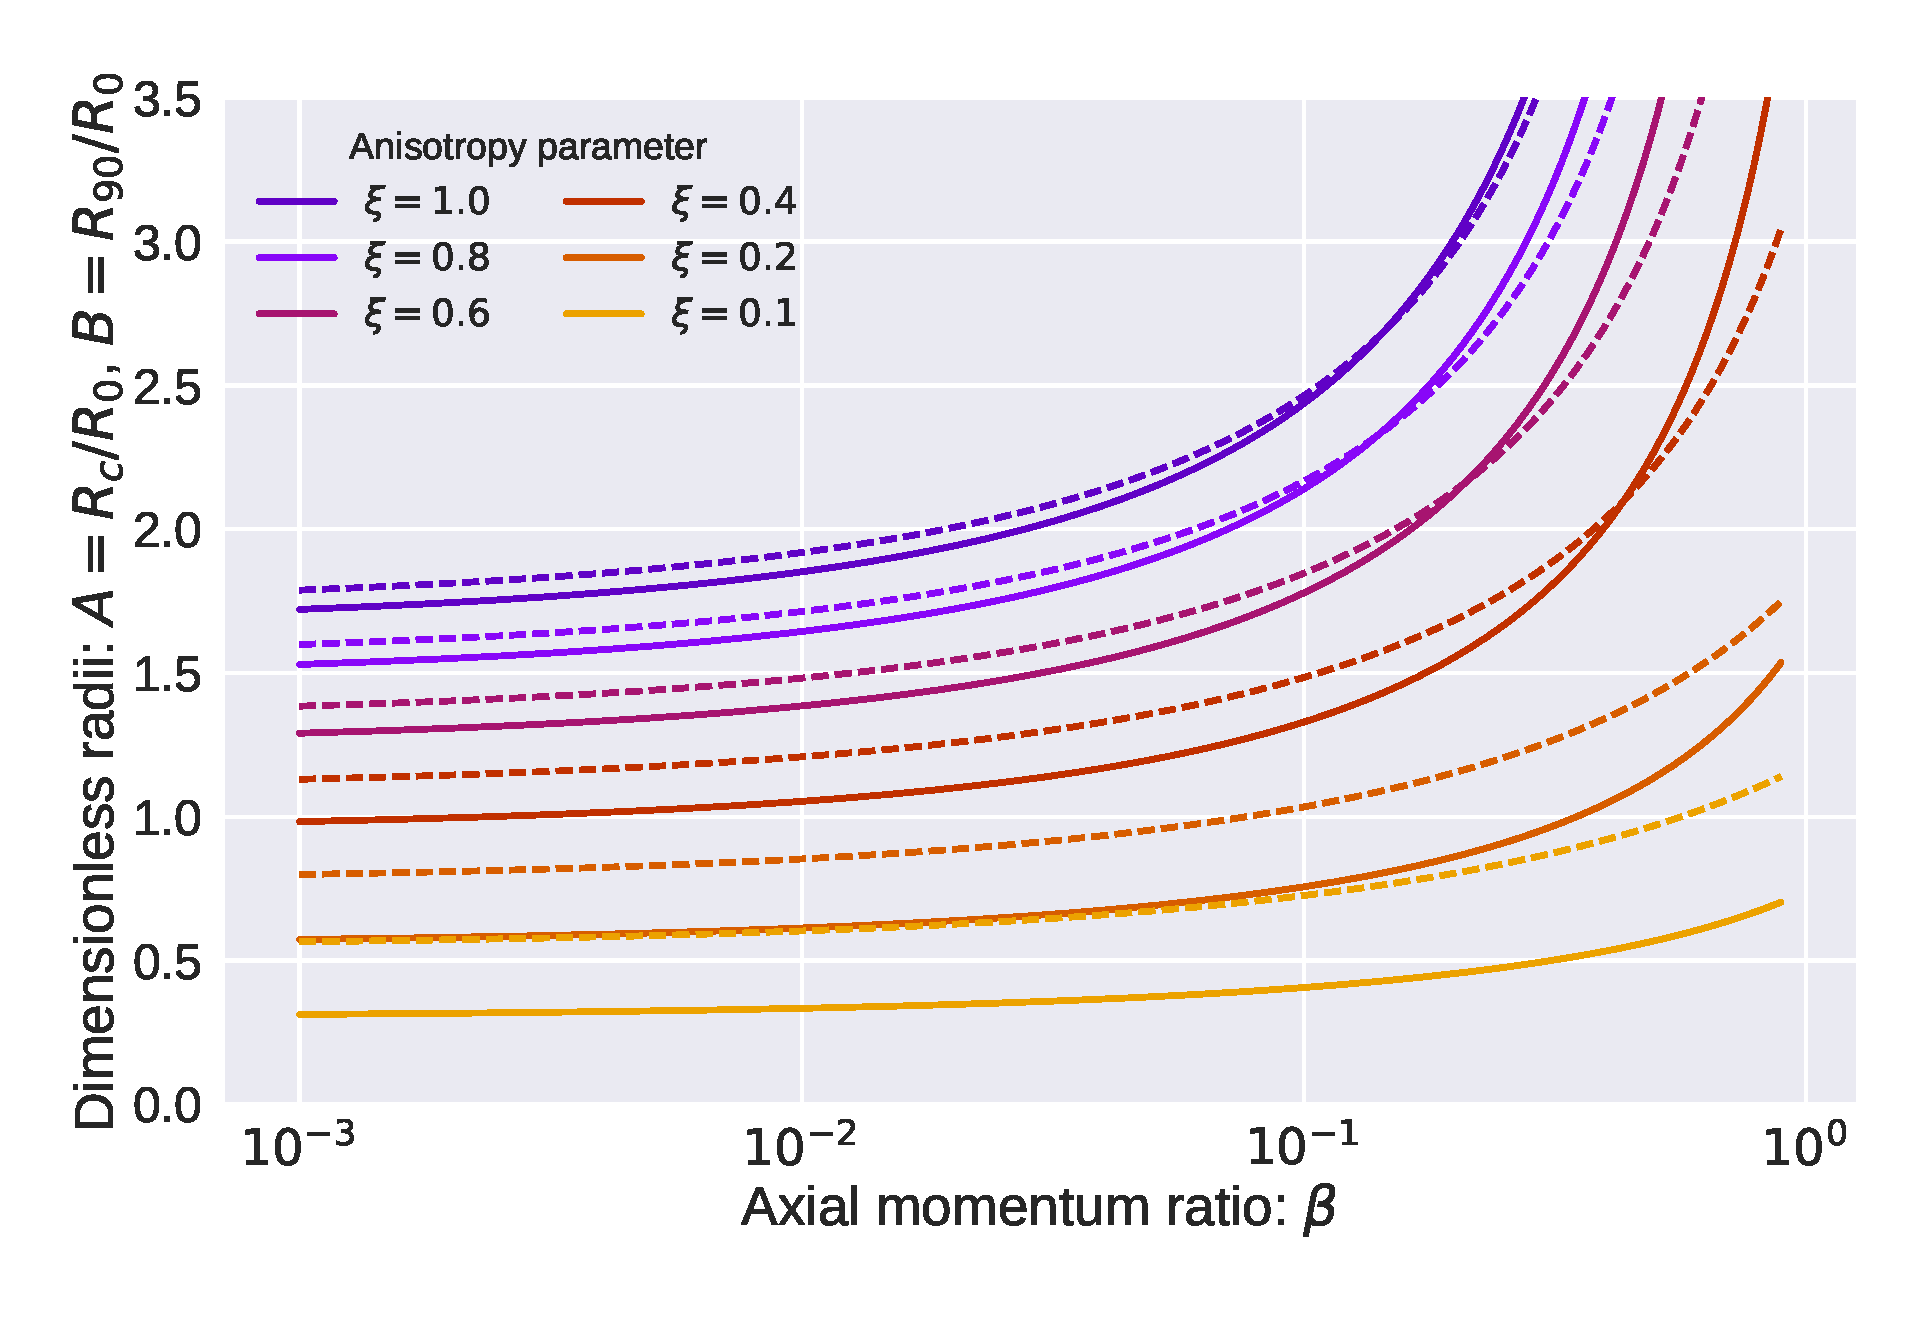
\includegraphics[width=\linewidth]{figs/AB-beta-log} \\
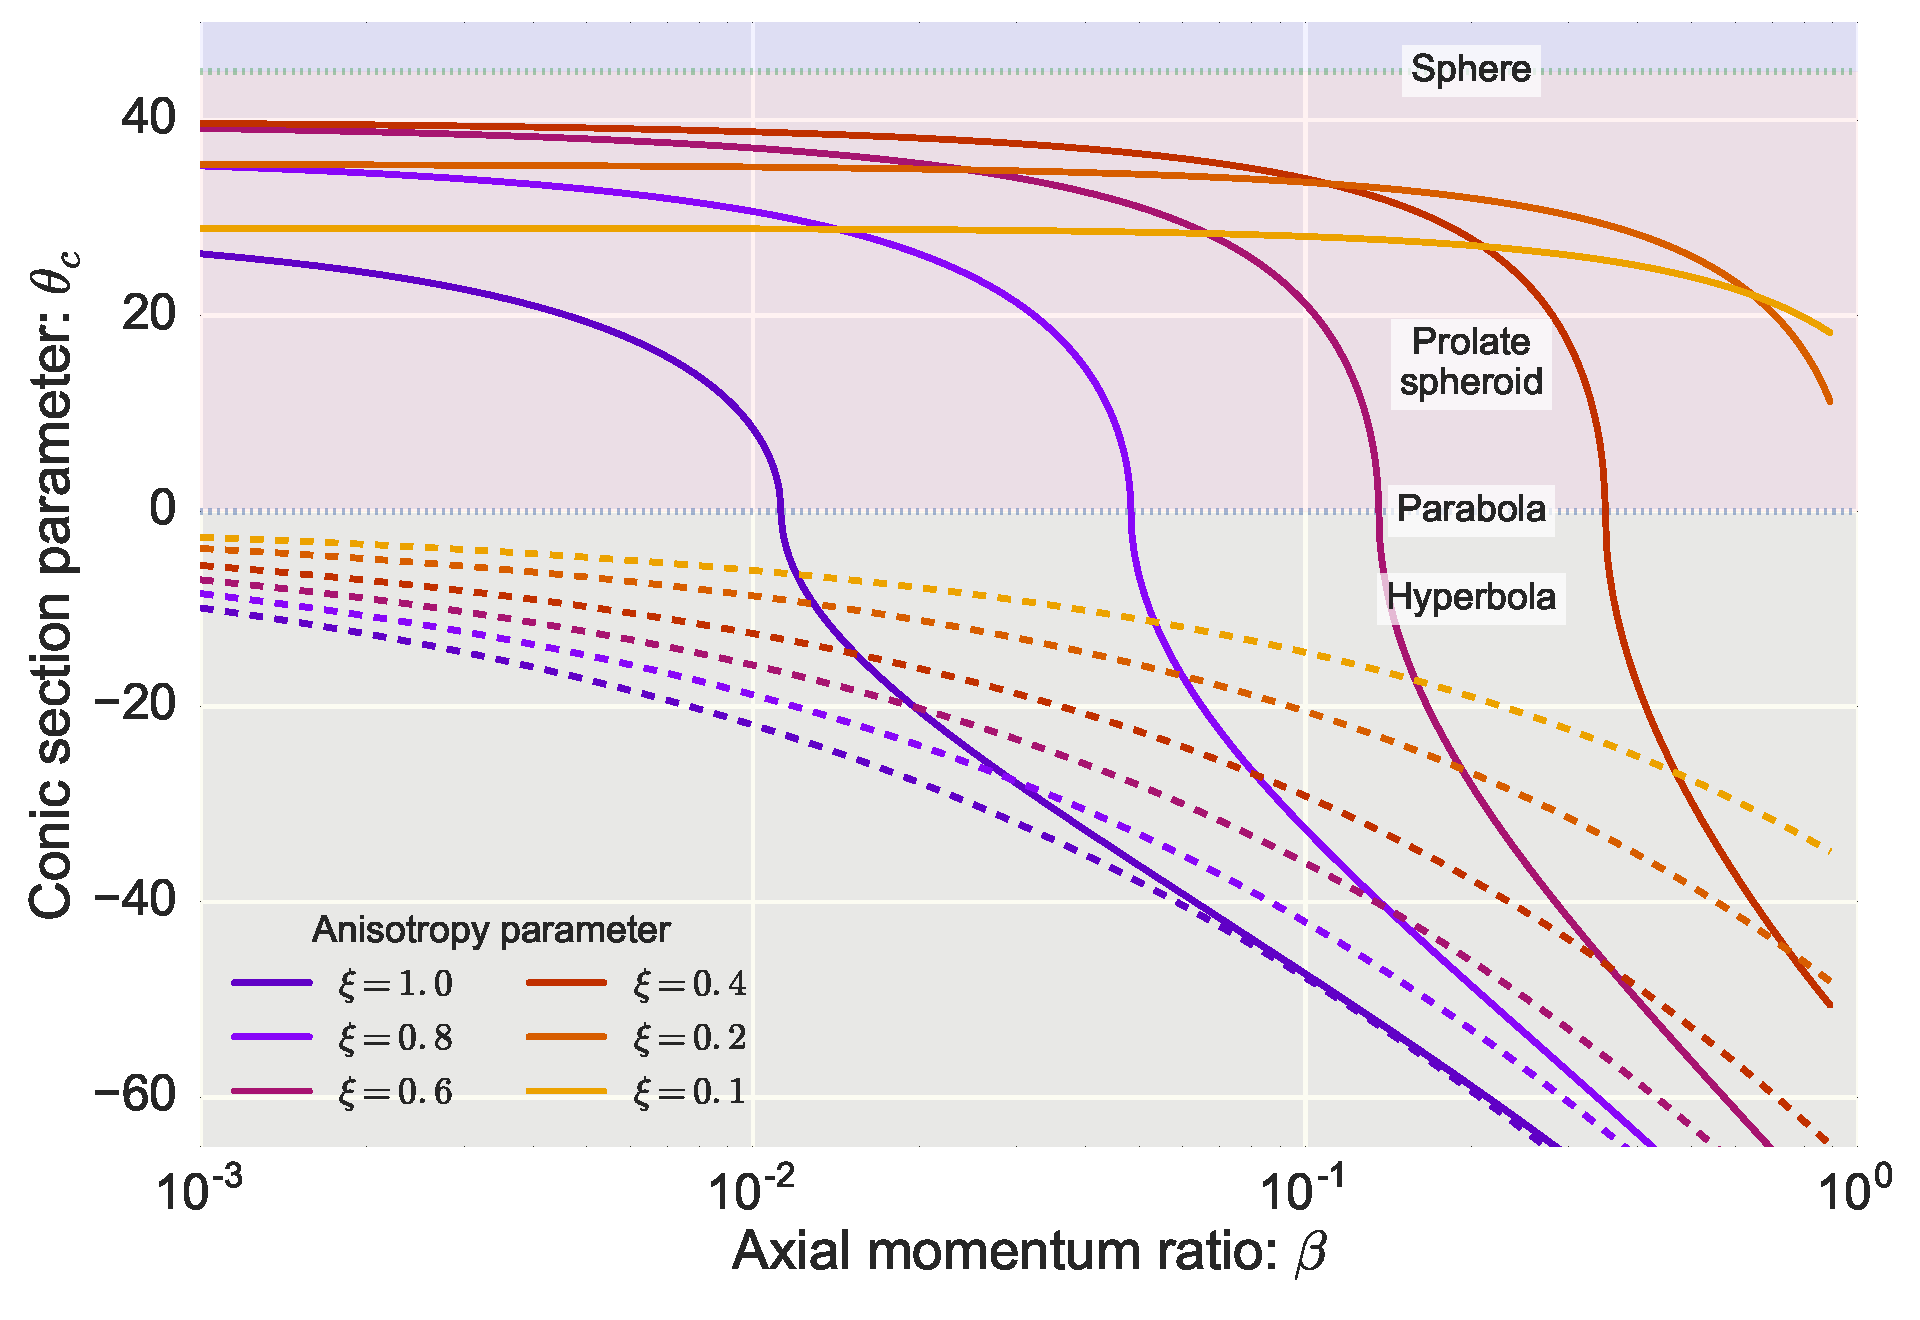
\includegraphics[width=\linewidth]{figs/thc-beta-log}
\end{tabular}
\caption{Top: Characteristic radii, $A = R_c/R_0$ (solid lines) and $B
  = R_{90}/R_0$ (dashed lines)
  vs $\beta$, calculated from quadric fits to the generalized CRW
  solutions with varying degrees of isotropy $\xi$.  Bottom: Conic
  angle $\theta_c$ vs $\beta$ for the bow 
  shock head (solid lines) and the bow shock tail (dashed lines).}
\label{fig:rad-beta}
\end{figure}


%Observationally, we can measure the projected radii. In order to estimate the model parameters is neccesary to measure at least two of the mentioned radii, being $R_0$ the
%easiest to measure. Therefore, we may compare both $R_c$ and $R_{90}$ against $R_0$ as shown in figure (\ref{fig:prop-shell-rad}). 

With this we can use the results of section \ref{sec:conic} to estimate the projected conic shapes for bow shocks with different winds 
momenta and different density distributions. Figure \ref{fig:rad-beta} shows equations ( \ref{eq:B}), (\ref{eq:Rcurv}) and (\ref{eq:thc-CRW}) for different anisotropy indexes. 




\begin{figure*}
  \centering
  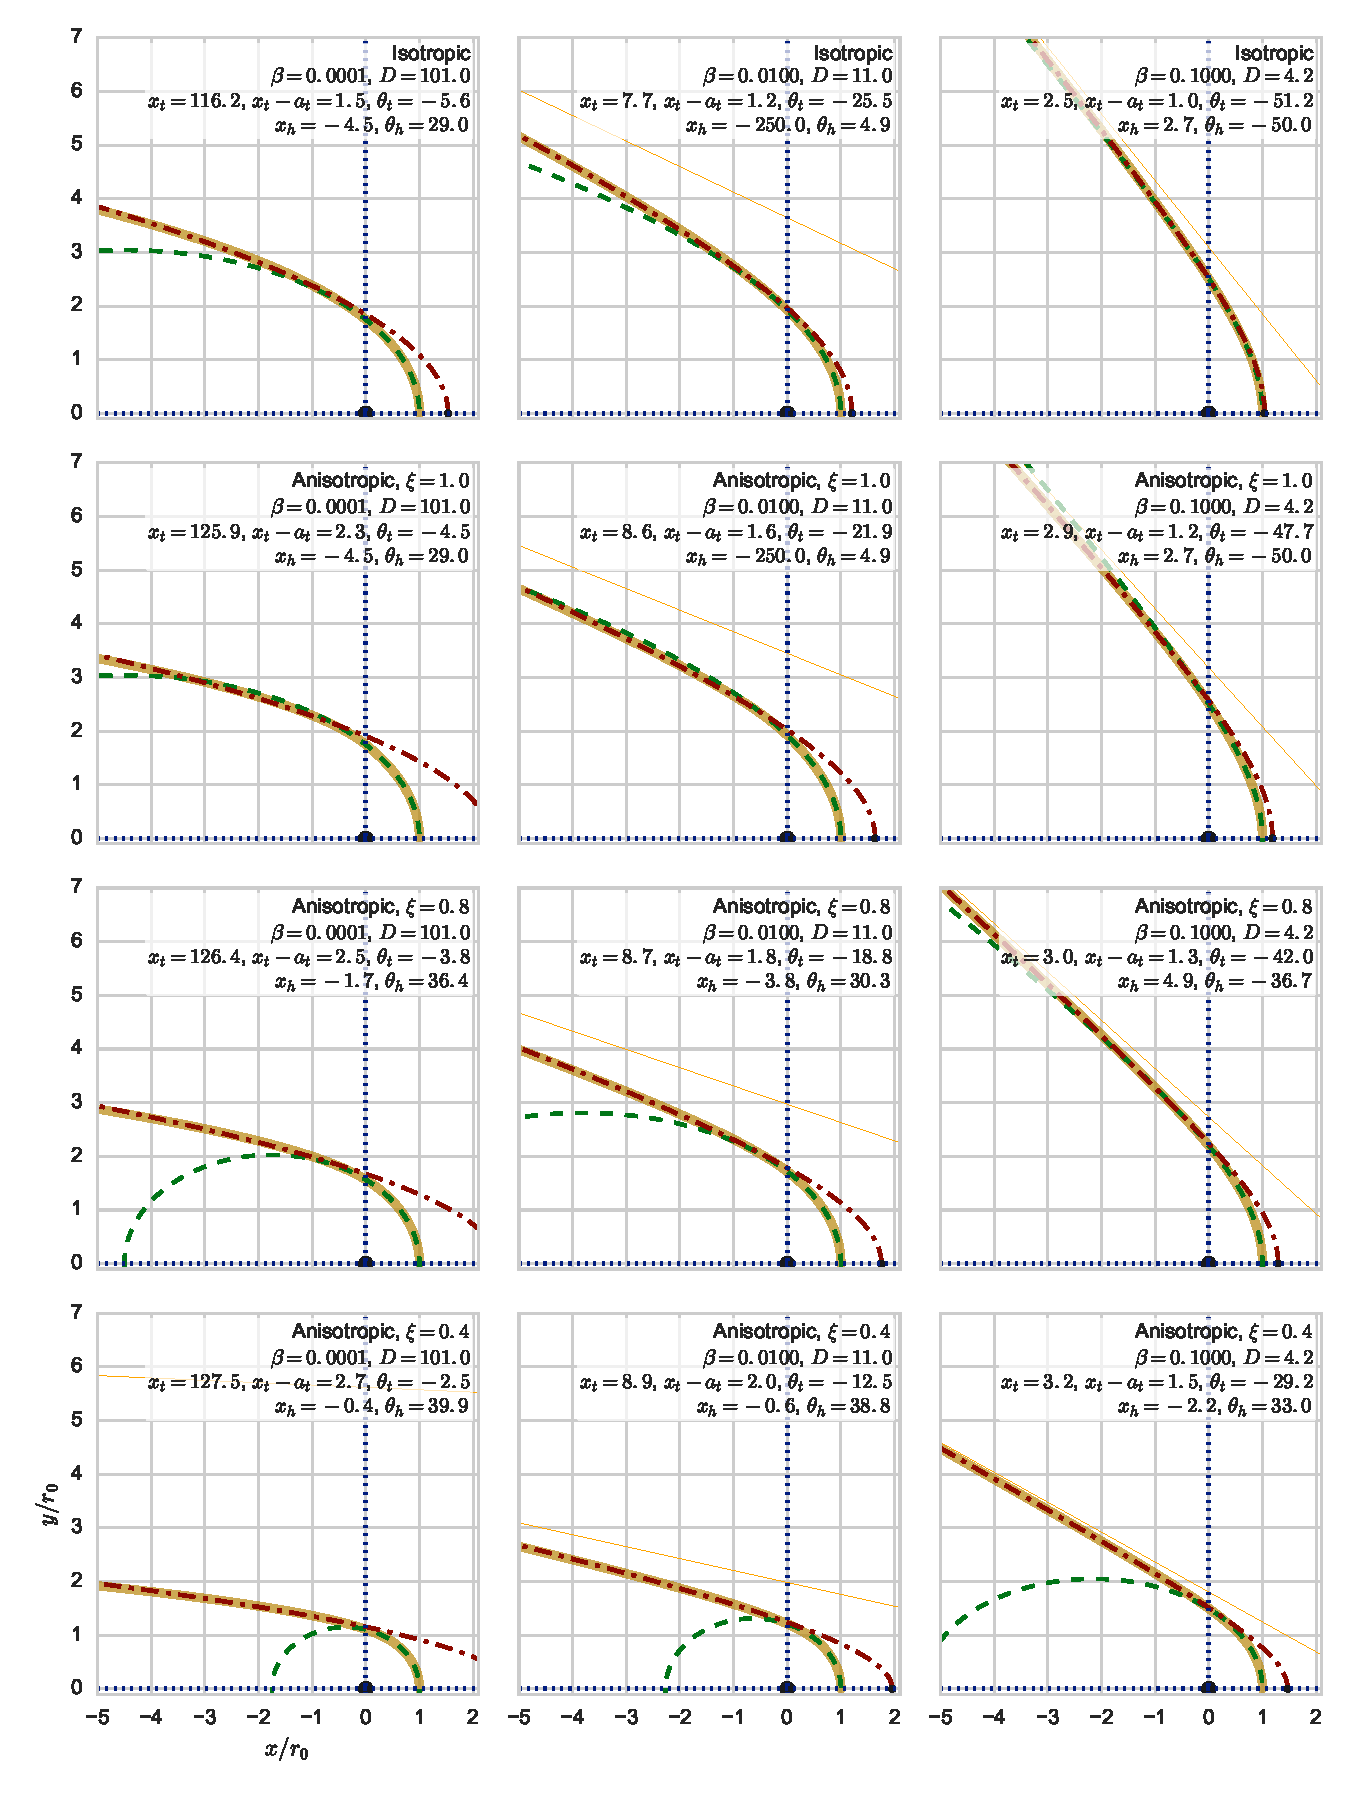
\includegraphics[width=\linewidth]{figs/conic-head-tail-fit}
  \caption{Double quadric fits to thin shell solutions.}
  \label{fig:head-tail}
\end{figure*}

%%% Local Variables:
%%% mode: latex
%%% TeX-master: "quadrics-bowshock"
%%% End:
